\begin{figure}[ht] \centering
    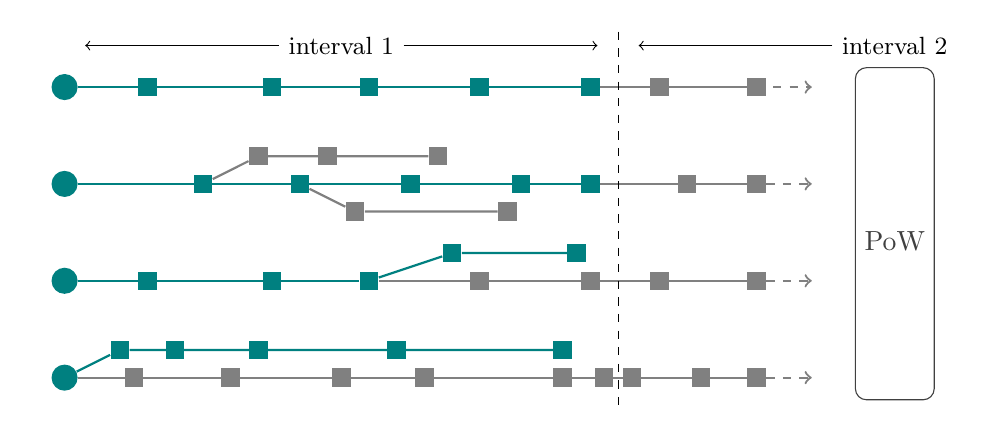
\begin{tikzpicture}
        \node (genesis) {};

        \node[fill = teal, circle] at ([xshift = 10pt, yshift = 50pt]genesis) (block11) {};
        \node[fill = teal] at ([xshift = 30pt]block11) (block12) {};
        \node[fill = teal] at ([xshift = 75pt]block11) (block13) {};
        \node[fill = teal] at ([xshift = 110pt]block11) (block14) {};
        \node[fill = teal] at ([xshift = 150pt]block11) (block15) {};
        \node[fill = teal] at ([xshift = 190pt]block11) (block16) {};
        \node[fill = gray] at ([xshift = 215pt]block11) (block17) {};
        \node[fill = gray] at ([xshift = 250pt]block11) (block1x) {};
        \draw[teal, thick] (block11) -- (block16);
        \draw[gray, thick] (block16) -- (block1x);

        \node[fill =  teal, circle] at ([xshift = 10pt, yshift = 15pt]genesis) (block21) {};
        \node[fill = teal] at ([xshift = 50pt]block21) (block22) {};
        \node[fill = teal] at ([xshift = 85pt]block21) (block23) {};
        \node[fill = teal] at ([xshift = 125pt]block21) (block24) {};
        \node[fill = teal] at ([xshift = 165pt]block21) (block25) {};
        \node[fill = teal] at ([xshift = 190pt]block21) (block26) {};
        \node[fill = gray] at ([xshift = 225pt]block21) (block27) {};
        \node[fill = gray] at ([xshift = 250pt]block21) (block2x) {};
        \draw[teal, thick] (block21) -- (block26);
        \draw[gray, thick] (block26) -- (block2x);
        \node[fill = gray] at ([xshift = 70pt, yshift = 10pt]block21) (block2f1) {};
        \node[fill = gray] at ([xshift = 95pt, yshift = 10pt]block21) (block2f2) {};
        \node[fill = gray] at ([xshift = 135pt, yshift = 10pt]block21) (block2f3) {};
        \draw[gray, thick] (block22) -- (block2f1) -- (block2f3);
        \node[fill = gray] at ([xshift = 105pt, yshift = -10pt]block21) (block2f4) {};
        \node[fill = gray] at ([xshift = 160pt, yshift = -10pt]block21) (block2f5) {};
        \draw[gray, thick] (block23) -- (block2f4) -- (block2f5);


        \node[fill =  teal, circle] at ([xshift = 10pt, yshift = -20pt]genesis) (block31) {};
        \node[fill = teal] at ([xshift = 30pt]block31) (block32) {};
        \node[fill = teal] at ([xshift = 75pt]block31) (block33) {};
        \node[fill = teal] at ([xshift = 110pt]block31) (block34) {};
        \node[fill = gray] at ([xshift = 150pt]block31) (block35) {};
        \node[fill = gray] at ([xshift = 190pt]block31) (block36) {};
        \node[fill = gray] at ([xshift = 215pt]block31) (block37) {};
        \node[fill = gray] at ([xshift = 250pt]block31) (block3x) {};
        \draw[teal, thick] (block31) -- (block34);
        \draw[gray, thick] (block34) -- (block3x);
        \node[fill = teal] at ([xshift = 140pt, yshift = 10pt]block31) (block3f1) {};
        \node[fill = teal] at ([xshift = 185pt, yshift = 10pt]block31) (block3f2) {};
        \draw[teal, thick] (block34) -- (block3f1) -- (block3f2);


        \node[fill =  teal, circle] at ([xshift = 10pt, yshift = -55pt]genesis) (block41) {};
        \node[fill = gray] at ([xshift = 250pt]block41) (block4x) {};
        \node[fill = gray] at ([xshift = 25pt]block41) (block42) {};
        \node[fill = gray] at ([xshift = 60pt]block41) (block43) {};
        \node[fill = gray] at ([xshift = 100pt]block41) (block44) {};
        \node[fill = gray] at ([xshift = 130pt]block41) (block45) {};
        \node[fill = gray] at ([xshift = 180pt]block41) (block46) {};
        \node[fill = gray] at ([xshift = 195pt]block41) (block47) {};
        \node[fill = gray] at ([xshift = 205pt]block41) (block48) {};
        \node[fill = gray] at ([xshift = 230pt]block41) (block49) {};
        \draw[gray, thick] (block41) -- (block4x);
        \node[fill = teal] at ([xshift = 20pt, yshift = 10pt]block41) (block4f1) {};
        \node[fill = teal] at ([xshift = 40pt, yshift = 10pt]block41) (block4f2) {};
        \node[fill = teal] at ([xshift = 70pt, yshift = 10pt]block41) (block4f3) {};
        \node[fill = teal] at ([xshift = 120pt, yshift = 10pt]block41) (block4f4) {};
        \node[fill = teal] at ([xshift = 180pt, yshift = 10pt]block41) (block4f5) {};
        \draw[teal, thick] (block41) -- (block4f1) -- (block4f5);

        \draw[black, dashed] ([xshift = 200pt, yshift = 20pt]block11.center) -- ([xshift = 200pt, yshift = -10pt]block41.center);
        \node at ([xshift = 100pt, yshift = 15pt]block11.center) (interval1) {\small interval 1};
        \draw[black, ->] (interval1.west) -- ([xshift = -70pt]interval1.west);
        \draw[black, ->] (interval1.east) -- ([xshift = 70pt]interval1.east);
        \node at ([xshift = 300pt, yshift = 15pt]block11.center) (interval2) {\small interval 2};
        \draw[black, ->] (interval2.west) -- ([xshift = -70pt]interval2.west);

        \node[darkgray, fill = white, draw = darkgray, rounded corners, minimum height = 120pt, align=center] at ([xshift = 50pt, yshift = -18pt]block2x) (pow) {\funcRO\\\mforone PoW};

        \draw[gray, thick, dashed, ->] (block1x.center) -- ([xshift = 20pt]block1x.center);
        \draw[gray, thick, dashed, ->] (block2x) -- ([xshift = 20pt]block2x.center);
        \draw[gray, thick, dashed, ->] (block3x) -- ([xshift = 20pt]block3x.center);
        \draw[gray, thick, dashed, ->] (block4x) -- ([xshift = 20pt]block4x.center);
    \end{tikzpicture}

    \caption{
        An illustration of the parallel blocktrees and the mining procedure.
        %
        Genesis blocks on each chain are represented as circles.
        %
        Teal blocks and forks depicts the view of a party at the end of the first interval.
        %
        There is no fork on the first chain; and on the second chain, forks are bookkeeped yet fail to revert the longest one.
        %
        The last two blocks in the view of a party on the third chain are discarded from the longest chain by another longer fork.
        %
        On the forth chain, all blocks in the first interval are reverted.
    }
    \label{fig:parallel-blocktree}
\end{figure}
